\chapter{荷電粒子、場の変換、相対論的波動}

前回、相対性原理を課したとき、荷電粒子が電場と磁場の中でどのように運動するかを問い始めた。よく知られたローレンツ力の法則にはすでに手がかりが含まれている。その磁気的な項は粒子の速度に依存するので、異なる観測者が何が電場で何が磁場であるかについて別々に一致することはできない。我々の課題は、場と粒子の速度が座標系ごとに変わるにもかかわらず、すべての慣性観測者が同じ方程式を用いるようにこの法則を定式化することである。

特に断らない限り、\(c=1\) と計量の符号 \((-,-,-,+)\) をとる単位系を用いる。時空の成分は三つの空間成分を先にして並べる：
\begin{equation}
  \mu=(1,2,3,0)=(x,y,z,t).
\end{equation}
ラテン添字 \(m,n\) は三つの空間方向のみを走る。

\section{ニュートンの力の法則から何が生き残るか}

ニュートン力学では、
\begin{equation}
  \boldsymbol F=m\boldsymbol a
\end{equation}
はガリレイ的観測者が加速度について一致するため、すべての慣性系で同じ形をとる。彼らはまた粒子に同じ質量と同じ力を割り当てる。運動学が変われば、力と通常の加速度の間のこの特定の関係がそのまま生き残ると期待する理由はない。

電磁気学と重力はすでに、相対論的拡張が互いに似ている必要はないことを警告している。クーロンの法則とニュートンの重力の法則はどちらも逆二乗の法則であるが、重力は時空の幾何学に深い変更を加えなければ特殊相対性理論に自然に組み込むことができない。電磁気学は組み込むことができる。実際、磁気はそれ自体が相対論的効果である。\(c\) の因子を復元すると、磁気力は速度を \(c\) で割った因子を伴い、形式的な極限 \(c\to\infty\) で消える。

ニュートンの法則の耐久性のある部分は、力が運動量の変化率であるという主張である。静止質量が一定の場合、
\begin{equation}
  \boldsymbol F
  =m\frac{d\boldsymbol v}{dt}
  =\frac{d}{dt}(m\boldsymbol v)
  =\frac{d\boldsymbol p}{dt}.
\end{equation}
相対性理論は運動量と速度の関係を変えるが、この方程式の整理の仕方は保存する。

\begin{figure}[H]
\centering
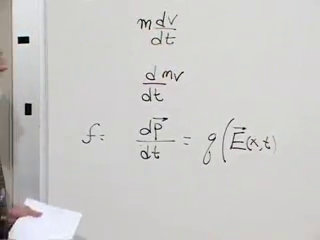
\includegraphics[width=0.64\textwidth]{lecture_07_figure_01.png}
\caption{ローレンツの法則の電気的な部分が黒板に書かれている間に、力を \(d\boldsymbol p/dt\) として書き直したもの。}
\lectureframe{00:08:20}
\end{figure}

単位 \(c=1\) では、相対論以前のローレンツ力の法則は
\begin{equation}
  \frac{d\boldsymbol p}{dt}
  =q\bigl(\boldsymbol E+\boldsymbol v\times\boldsymbol B\bigr).
  \label{eq:lorentz-three}
\end{equation}
である。両方の場は位置と時間に依存してよい。非相対論的極限は今や \(v\ll 1\) の極限であり、数値定数 \(c=1\) が何らかの形で変化する極限ではない。\eqref{eq:lorentz-three} の電気的な項はすでに通常のベクトルである。磁気的な項を時空に持ち込める形で理解するには、外積をもう一度見なければならない。

\section{反対称テンソルとしての外積}

二つの三次元ベクトル \(\boldsymbol A\) と \(\boldsymbol B\) をとる。それらの外積
\begin{equation}
  T_{mn}=A_mB_n
\end{equation}
は九つの成分をもつ二階のテンソルである。一般には対称性をもたない。反対称化すると
\begin{equation}
  K_{mn}=A_mB_n-A_nB_m,
  \qquad K_{mn}=-K_{nm}.
  \label{eq:antisym-product}
\end{equation}
が得られる。対角成分は消え、対角より下の各成分はそれに対応する上の成分によって定まる。したがって \(3\times3\) の反対称テンソルは三つの独立な成分しかもたない。

この数え上げは示唆的であるが、それだけでは十分ではない。三つの量が自動的にベクトルとして変換するわけではない。しかし三次元では、\eqref{eq:antisym-product} の三つの独立な成分を外積
\(\boldsymbol C=\boldsymbol A\times\boldsymbol B\) の成分と同一視することができる。黒板ではまず \(C_2\) を右上の位置に暫定的に置く：

\begin{figure}[H]
\centering
\includegraphics[width=0.75\textwidth]{lecture_07_figure_02.png}
\caption{その三つの独立な成分が \(\boldsymbol C\) の成分と対応づけられている間の反対称積。ここでは右上のラベルはまだ暫定的である。}
\lectureframe{00:17:33}
\end{figure}

\(1\to2\to3\to1\) を巡回させると成分の公式
\begin{align}
  C_3 &= A_1B_2-A_2B_1, \\
  C_1 &= A_2B_3-A_3B_2, \\
  C_2 &= A_3B_1-A_1B_3.
  \label{eq:cross-components}
\end{align}
が得られる。最後の行は、右上の成分が \(C_2\) ではなく \(-C_2\) であることを示している。この修正は隠すべき細部ではなく、議論の一部である。

\begin{figure}[H]
\centering
\includegraphics[width=0.62\textwidth]{lecture_07_figure_03.png}
\caption{反対称配列における暫定的な符号を確定する、完成した巡回的な成分の恒等式。}
\lectureframe{00:21:54}
\end{figure}

得られる行列は
\begin{equation}
  K_{mn}=
  \begin{pmatrix}
    0 & C_3 & -C_2 \\
    -C_3 & 0 & C_1 \\
    C_2 & -C_1 & 0
  \end{pmatrix}.
  \label{eq:cross-matrix}
\end{equation}
である。

この記法の背後には有用な幾何学がある。添字 \(1,2\) をもつ成分は自然に \(xy\) 平面に属し、それに垂直な \(z\) 軸に沿ったベクトル成分と同一視される。同じ向きづけられた対象を、平面によって記述しても、その平面に垂直な矢印によって記述してもよい。矢印による記述は三次元に特有である。より高い次元では反対称二階テンソルは依然として存在するが、もはやベクトルと同じ数の成分をもたない。したがって一般化するのは垂直な矢印ではなく、テンソルのほうである。

同値的には、向きを選んだ後で、
\begin{equation}
  C_k=\frac12\epsilon_{kmn}K_{mn}.
\end{equation}
向きを選ぶ必要があることが、右手の法則と、極性ベクトルと軸性ベクトルの間のよく知られた区別の源である。
\editorialnote{Levi--Civitaの公式と軸性ベクトルという用語は、講義で明示的に展開された平面対法線の幾何学に対する標準的な記法である。}

\section{テンソル形式の磁場}

同じ双対的な記述が磁場にも当てはまる。その反対称空間テンソルを次で定義する：
\begin{equation}
  B_{mn}=
  \begin{pmatrix}
    0 & -B_3 & B_2 \\
    B_3 & 0 & -B_1 \\
    -B_2 & B_1 & 0
  \end{pmatrix}.
  \label{eq:magnetic-tensor}
\end{equation}
\eqref{eq:cross-matrix}に対する余分な全体符号は慣習である。ひとたびそれを選べば、一貫して用いなければならない；三つのベクトル成分すべての符号を変えることは、反対の向きの慣習で同じテンソルとベクトルの同一視を記述することになる。

\begin{figure}[H]
\centering
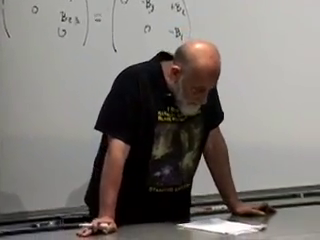
\includegraphics[width=0.72\textwidth]{lecture_07_figure_04.png}
\caption{反対称空間配列として、またその三つのベクトル成分によって書かれた磁場。}
\lectureframe{00:24:40}
\end{figure}

次に、クロス積の第3成分を取る：
\begin{align}
  (\boldsymbol v\times\boldsymbol B)_3
  &=v_1B_2-v_2B_1 \\
  &=v_1B_{13}+v_2B_{23}+v_3B_{33}.
\end{align}
最後の項は\(B_{33}=0\)であるため加えることができる。自由成分を巡回させると、次の簡潔な規則が得られる：
\begin{equation}
  (\boldsymbol v\times\boldsymbol B)_m=v_nB_{nm},
  \label{eq:cross-contraction}
\end{equation}
ここで、繰り返される添字\(n\)は和を取る。したがって、磁気力は
\begin{equation}
  F_m^{(B)}=qv_nB_{nm}.
\end{equation}

\begin{figure}[H]
\centering
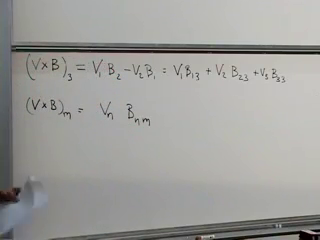
\includegraphics[width=0.78\textwidth]{lecture_07_figure_05.png}
\caption{\(\boldsymbol v\times\boldsymbol B\)の第3成分と、\(B_{nm}\)との縮約としてのその一般式。}
\lectureframe{00:28:30}
\end{figure}

\begin{classroomqa}
\audiencequestion{自由添字\(m\)は力の別個の磁気成分を表すのか？}
\lecturerresponse{いいえ。それは、計算されている力の空間成分を表す。電場は現在の議論のために単にゼロに設定されており、ここでのすべての添字は三つの空間方向にのみ走る。}
\end{classroomqa}

テンソル記法は、磁場の仕事をしない性質をほとんど自動的にする。速度の二乗を微分する：
\begin{align}
  \frac{d}{dt}(v_mv_m)
  &=2\dot v_m v_m \\
  &\propto 2(\boldsymbol v\times\boldsymbol B)_m v_m \\
  &=2v_nB_{nm}v_m.
  \label{eq:speed-derivative}
\end{align}
\(m=n\)を含む項は、\(B_{nm}\)の対角成分がゼロであるため消える。すべての非対角項には、\(m\)と\(n\)を入れ替えた相棒があり、\(v_nv_m\)は対称である一方で\(B_{nm}\)は反対称であるため、二つは相殺する。したがって
\begin{equation}
  \frac{d}{dt}(v_mv_m)=0.
\end{equation}
純粋な磁気力は、速度や運動エネルギーを変えずに軌道を曲げる。

\begin{figure}[H]
\centering
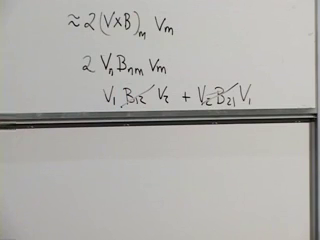
\includegraphics[width=0.68\textwidth]{lecture_07_figure_06.png}
\caption{\(v_nB_{nm}v_m\)の対になった項は、磁気テンソルが添字を入れ替えると符号を変えるため相殺する。}
\lectureframe{00:35:40}
\end{figure}

この証明は、クロス積がその最初の因子に垂直であると言うよりも意図的に手が込んでいる。後者の言明は三次元ベクトル表現に特有である。対称な対と反対称テンソルの縮約が、四次元でも生き残る議論である。

\begin{classroomqa}
\audiencequestion{速度が一定に保たれるためには、磁場は時間に依存してはならないのか？}
\lecturerresponse{上記の代数は場を微分することはなく、\(\partial_t\boldsymbol B=0\)を必要としない。磁気項だけでも依然として仕事をしない。しかし、電気力学では、変化する磁場が電場を生み、その電場が粒子の速度を変えうる。}
\end{classroomqa}

\section{なぜ電場と磁場は混ざり合わなければならないのか}

\(\boldsymbol E\)と\(\boldsymbol B\)の混合は、四次元計算の前に見ることができる。通常のニュートン的な加速度についての言明が十分であるような遅い運動を考える。磁場が\(y\)軸に沿っており、荷電粒子が\(x\)軸に沿って運動するとする。磁気力は\(z\)軸に沿って向く：
\begin{equation}
  \boldsymbol F=q\boldsymbol v\times\boldsymbol B.
\end{equation}

\begin{figure}[H]
\centering
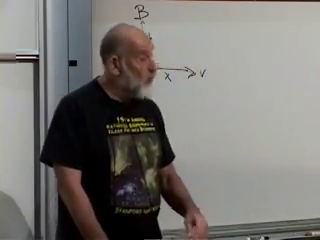
\includegraphics[width=0.62\textwidth]{lecture_07_figure_07.png}
\caption{磁場を横切って運動する粒子のための板書スケッチ；三つの方向は実験室と共動の記述を比較するために用いられる。}
\lectureframe{00:42:20}
\end{figure}

この幾何学は教室の遠近法なしで描き直すことができる：
\begin{figure}[H]
\centering
\begin{tikzpicture}[scale=1.05,>=Stealth]
  \draw[->] (0,0) -- (3.8,0) node[right] {\(x\)};
  \draw[->] (0,0) -- (-1.9,2.4) node[above left] {\(y\)};
  \draw[->] (0,0) -- (0,3.1) node[above] {\(z\)};
  \draw[->,very thick] (0,0) -- (2.7,0)
    node[midway,below] {\(\boldsymbol v\)};
  \draw[->,very thick] (0,0) -- (-1.35,1.7)
    node[midway,above left] {\(\boldsymbol B\)};
  \draw[->,very thick] (0,0) -- (0,2.35)
    node[midway,right] {\(\boldsymbol F,\ \boldsymbol E'\)};
\end{tikzpicture}
\caption{実験室では\(z\)方向の力は磁気的である；瞬間的な共動系では同じ力は電気的でなければならない。}
\end{figure}

次に、その瞬間に粒子とともに運動する観測者を導入する。新しい系での粒子の速度はゼロであるため、磁気項\(q\boldsymbol v'\times\boldsymbol B'\)は消える。しかし、遅い運動の極限では、両方の観測者が粒子が\(z\)加速度を持つことに同意しなければならない。ローレンツ力の法則が両方の系で同じ形を持つならば、共動観測者は力を\(z\)に沿った電場\(\boldsymbol E'\)に帰さなければならない。したがって、実験室で純粋に磁気的であった場は、運動系では純粋に磁気的ではない。

これが、両方の場を成分に含む単一の対象を求めるべき物理的な理由である。座標系の変更は、\(\boldsymbol E\) をそれ自身の3つの成分の間で回転させ、\(\boldsymbol B\) をそれ自身の3つの成分の間で回転させるだけではなく、2つの組を混合する。

\section{電磁場テンソル}

電場と磁場を合わせると6つの成分をもつ。4次元反対称テンソルもまた6つの独立な成分をもつ。なぜなら
\begin{equation}
  \frac{4(4-1)}{2}=6.
\end{equation}
これは、反対称テンソルが文字通り発明できる唯一の6つの量の集まりであることを意味しない。6つのスカラー、あるいはベクトルと2つのスカラーもまた6つの数を含むであろう。それは、その成分が必要とされる仕方で混合しうる自然な幾何学的対象である。

板書の規約を明示するために、反変テンソルを空間優先の順序 \((1,2,3,0)\) で表示する：
\begin{equation}
  F^{\mu\nu}=
  \begin{pmatrix}
    0 & -B_3 & B_2 & E_1 \\
    B_3 & 0 & -B_1 & E_2 \\
    -B_2 & B_1 & 0 & E_3 \\
    -E_1 & -E_2 & -E_3 & 0
  \end{pmatrix}.
  \label{eq:l07-field-tensor}
\end{equation}
左上の \(3\times3\) ブロックはまさに磁気テンソル \eqref{eq:magnetic-tensor} である。1つの空間指数と1つの時間指数をもつ成分は電場を含む。反対称性が残りの成分を与える。

\begin{figure}[H]
\centering
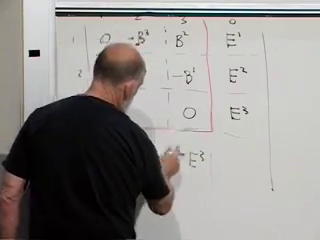
\includegraphics[width=0.72\textwidth]{lecture_07_figure_08.png}
\caption{磁気的な空間ブロックと電気的な時間-空間列が4次元場テンソルへと組み立てられる。}
\lectureframe{00:46:35}
\end{figure}

\begin{classroomqa}
\audiencequestion{これらの場の成分はいつ上付き指数をもつべきで、いつ下付き指数をもつべきか。}
\lecturerresponse{3つの空間ラベルだけについては、板書ではなじみ深いマクスウェル--ファラデー場を同定する際にその区別を省略することがある。共変的な計算ではその区別を復元しなければならない。空間指数を上げたり下げたりすることは、選ばれた計量規約において符号を変える。}
\end{classroomqa}

不変なのは、板書上の特定の符号の配置ではなく、反対称時空テンソルと、整合した計量および指数規約の組み合わせである。表記 \(F\) はファラデーを連想させるかもしれないが、講義はその歴史的帰属を自信をもって主張しているわけではない。アインシュタインは 1905 年に電場と磁場の成分の変換を導いた。コンパクトな4次元テンソル言語は、ミンコフスキーに結びつけられる後期の時空定式化とともに現れた。

\section{4元速度と4元力}

方程式の粒子側も共変的にしなければならない。固有時 \(\tau\) は不変であるから、位置4元ベクトルをそれで微分すると別の4元ベクトルが得られる：
\begin{equation}
  u^\mu=\frac{dx^\mu}{d\tau}
  =\gamma(v_x,v_y,v_z,1),
  \qquad
  \gamma=\frac{1}{\sqrt{1-v^2}}.
  \label{eq:four-velocity}
\end{equation}
最後の成分は \(dt/d\tau=\gamma\) から従う。4元運動量は
\begin{equation}
  p^\mu=mu^\mu,
\end{equation}
であり、その空間部分は相対論的運動量
\(\boldsymbol p=m\gamma\boldsymbol v\)
である。

\begin{figure}[H]
\centering
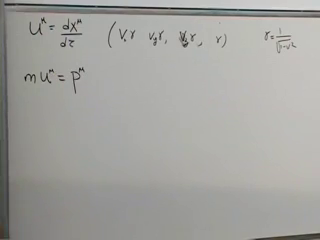
\includegraphics[width=0.75\textwidth]{lecture_07_figure_09.png}
\caption{4元速度、その成分、ローレンツ因子、および4元運動量。}
\lectureframe{00:50:30}
\end{figure}

\(p^\mu\) は4元ベクトルであり \(\tau\) はスカラーであるから、自然な相対論的左辺は
\begin{equation}
  f^\mu\equiv\frac{dp^\mu}{d\tau}.
  \label{eq:four-force-def}
\end{equation}
である。4元力は任意に選ぶことはできない。4元速度は固定されたノルムをもち、
\begin{equation}
  u_\mu u^\mu=1.
\end{equation}
世界線に沿って微分すると
\begin{align}
  0
  &=\frac{d}{d\tau}(u_\mu u^\mu) \\
  &=\frac{du_\mu}{d\tau}u^\mu
    +u_\mu\frac{du^\mu}{d\tau} \\
  &=2u_\mu\frac{du^\mu}{d\tau}.
\end{align}
が得られる。質量が一定の場合、これは
\begin{equation}
  f^\mu u_\mu=0.
  \label{eq:force-orthogonal}
\end{equation}
を意味する。したがって4元力は4元速度にミンコフスキー直交する。これは \(u^\mu\) の規格化から従う純粋に運動学的な制約であり、電磁気学に特有の性質ではない。

\begin{figure}[H]
\centering
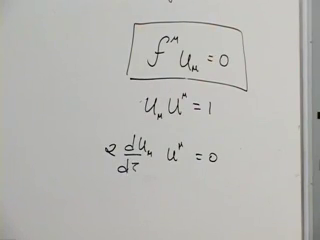
\includegraphics[width=0.64\textwidth]{lecture_07_figure_10.png}
\caption{4元速度の単位ノルムと、それから従う4元力と4元速度の直交性。}
\lectureframe{00:56:50}
\end{figure}

3次元の磁気的計算はすでに \eqref{eq:force-orthogonal} を満たすための仕掛けを与えている。反対称テンソルを速度の1つのコピーと縮約する：
\begin{equation}
  \boxed{
  \frac{dp^\mu}{d\tau}=qF^{\mu\nu}u_\nu.}
  \label{eq:covariant-lorentz}
\end{equation}
実際、
\begin{equation}
  f^\mu u_\mu
  =qF^{\mu\nu}u_\nu u_\mu=0,
\end{equation}
なぜなら \(F^{\mu\nu}\) は反対称であり、\(u_\nu u_\mu\) は対称だからである。これは考えうる唯一の相対論的力の法則ではないが、電磁場と速度の両方について線形な最も単純なものである。

\begin{figure}[H]
\centering
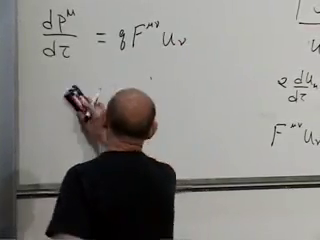
\includegraphics[width=0.72\textwidth]{lecture_07_figure_11.png}
\caption{左辺に共変的なローレンツ力方程式、右辺に第2の4元速度との消える縮約。}
\lectureframe{01:00:00}
\end{figure}

\section{通常のローレンツ力の回復}

共変的に見える方程式は、なお既知の力の法則を再現しなければならない。冒頭で述べた計量規約のもとで、
\begin{equation}
  u_\mu=\gamma(-v_x,-v_y,-v_z,1).
\end{equation}
\(x\) 成分については、\eqref{eq:l07-field-tensor} と
\eqref{eq:covariant-lorentz} から
\begin{align}
  \frac{dp^1}{d\tau}
  &=q\bigl(F^{12}u_2+F^{13}u_3+F^{10}u_0\bigr) \\
  &=q\gamma\bigl(B_3v_y-B_2v_z+E_1\bigr) \\
  &=q\gamma\bigl[\boldsymbol E+\boldsymbol v\times
    \boldsymbol B\bigr]_x.
  \label{eq:x-force}
\end{align}
が得られる。他の空間成分は指数を巡回させることで従う。

\begin{classroomqa}
\audiencequestion{成分展開における \(qE_x\) の項はどこにあるのか。}
\lecturerresponse{それは \(qF^{10}u_0\) の項である。1つの空間指数と1つの時間指数をもつ場テンソルの成分は電場の成分であり、\(u_0=\gamma\) である。}
\end{classroomqa}

右辺の因子 \(\gamma\) は余分な力ではない。
\begin{equation}
  \frac{dp^i}{d\tau}=\frac{dt}{d\tau}\frac{dp^i}{dt}
  =\gamma\frac{dp^i}{dt},
\end{equation}
であるから、\eqref{eq:x-force} の両辺から消える。したがって正確な空間方程式は再び
\begin{equation}
  \frac{d\boldsymbol p}{dt}
  =q\bigl(\boldsymbol E+\boldsymbol v\times\boldsymbol B\bigr),
  \qquad
  \boldsymbol p=m\gamma\boldsymbol v.
  \label{eq:exact-three-force}
\end{equation}
である。なじみ深い形は生き残るが、相対論は運動量の中に隠れている。

\begin{figure}[H]
\centering
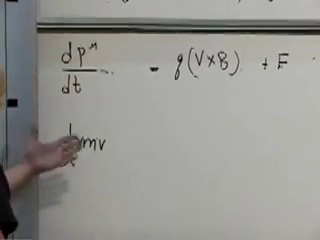
\includegraphics[width=0.75\textwidth]{lecture_07_figure_12.png}
\caption{共通の固有時因子を取り除いた後に三次元のローレンツ則が回復される。運動量は\(\gamma\)の因子を保持する。}
\lectureframe{01:06:30}
\end{figure}

時間成分は対応するエネルギーに関する命題を担い、
\begin{equation}
  \frac{dp^0}{dt}=q\boldsymbol E\cdot\boldsymbol v,
\end{equation}
したがって磁場は仕事をせず、電場は粒子のエネルギーを変化させうる。
\editorialnote{時間成分の検証は、この講義の空間的計算の直接の相棒である。これは同じ「仕事をしない」性質を四次元表記で明らかにするために含められている。}

\begin{classroomqa}
\audiencequestion{この導出は数学か物理か。}
\lecturerresponse{その両方である。テンソル代数が簡潔な形を与えるが、実質的な物理は、すべての慣性系が同じ法則に従うという原理と、運動方程式が二階であるという仮定を通じて入ってくる。二階の法則は位置と速度から未来を予測する。三階の法則ならば、加速度を追加の初期データとして必要とするだろう。自然がどちらの種類の法則を用いるかは、表記ではなく実験が教えてくれる。}
\end{classroomqa}

\section{場はどのように変換するか}

式\eqref{eq:covariant-lorentz}は、両辺が四元ベクトルであるため、どの慣性系でも同じ形をとる。場のテンソル自身は、各添字に一つずつローレンツ行列を掛けて変換する：
\begin{equation}
  F'^{\mu\nu}
  =\Lambda^\mu{}_{\rho}\Lambda^\nu{}_{\sigma}F^{\rho\sigma}.
  \label{eq:tensor-transform}
\end{equation}
黒板では、まず簡単な積\(A^\mu B^\nu\)を変換することによってこの規則を導く。ベクトルの積について規則がわかれば、線形性により任意の二階テンソルの規則が得られる。

\(1\)軸に沿ったブーストに対して、座標は次のように変換する：
\begin{align}
  x'^1&=\gamma(x^1-vx^0), &
  x'^0&=\gamma(x^0-vx^1), \\
  x'^2&=x^2, & x'^3&=x^3.
\end{align}
同じ変換を二つのテンソル添字に別々に適用する。ブーストに平行な成分について、黒板では積から始める：
\begin{align}
  (A'^0B'^1)
  =\gamma^2\bigl(
     A^0B^1-vA^0B^0-vA^1B^1+v^2A^1B^0
   \bigr).
\end{align}
各積を対応するテンソル成分に置き換え、次に反対称性\(F^{00}=F^{11}=0\)および\(F^{10}=-F^{01}\)を用いると、
\begin{equation}
  F'^{01}
  =\gamma^2(1-v^2)F^{01}
  =F^{01}.
\end{equation}
が得られる。したがって、運動に平行な電場成分は変わらない。平行な磁場成分も同様に振る舞う。

横成分は異なる。黒板で用いられたプライム系と符号の規約に従うと、
\begin{align}
  F'^{02}
  &=\gamma\bigl(F^{02}-vF^{12}\bigr), \\
  E'_2
  &=\gamma(E_2+vB_3).
  \label{eq:e-transform}
\end{align}
横電場成分は磁場成分の一部を獲得する。残りの変換則は同じ二添字規則から従い、講義の演習として残される。

\begin{figure}[H]
\centering
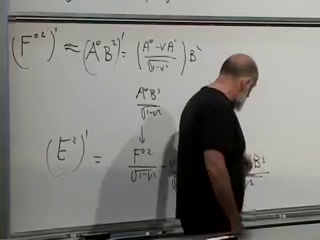
\includegraphics[width=0.76\textwidth]{lecture_07_figure_13.png}
\caption{\(E'_2\)成分が\(vB_3\)に比例する項を含むことがわかる点における横テンソル変換。}
\lectureframe{01:23:40}
\end{figure}

\eqref{eq:e-transform}における符号は、どちらの系が\(+v\)とともに動くと宣言されるか、また添字と計量の規約に依存する。その不変な内容は依存しない。横電場成分と横磁場成分は混合し、共変な力の方程式は変換後も有効である。

\begin{classroomqa}
\audiencequestion{ワイヤー中の電流について、磁場が消えるような速度で動くことはできるか。}
\lecturerresponse{伝導電子とともに動くだけでは十分でない。なぜなら、正の格子電荷が新しい系では動くからである。したがって、中性の電流を運ぶワイヤーは、単一の動く電荷の塊よりも微妙である。純粋に磁気的な場を完全に変換して消すことはできない。電場と磁場が両方存在する場合、それらの変換された部分は特別な状況で相殺しうる。一様に運動する一つの電荷については、その電荷の静止系が磁場の消える簡単な系である。}
\end{classroomqa}

正確な不変な判定は次を用いる：
\begin{equation}
  \boldsymbol B^2-\boldsymbol E^2,
  \qquad
  \boldsymbol E\cdot\boldsymbol B.
\end{equation}
\(\boldsymbol B'=0\)となる系は、\(\boldsymbol E\cdot\boldsymbol B=0\)である電場優勢の場に対してのみ存在しうる。ある系で純粋に磁気的な場は磁場優勢であり、その条件を満たすことはできない。
\editorialnote{これらの不変な判定基準は、教室での議論で到達した限定を正確に述べている。その導出は後回しにされる。}

\begin{classroomqa}
\audiencequestion{電気スカラーポテンシャルと磁気ベクトルポテンシャルは四元ベクトルをなすか。}
\lecturerresponse{はい。規約に依存する符号とともに、それらは四元ポテンシャル\(A^\mu\)に結合する。マクスウェル方程式はその対象を体系的に用いるであろう。}
\end{classroomqa}

\section{場の微分}

ここで一つの粒子の軌道を離れ、時空全体にわたる場を考える。
\begin{equation}
  \phi=\phi(x^1,x^2,x^3,x^0)
\end{equation}
をスカラー場とする。その四つの微分は四元ベクトルの共変成分をなす：
\begin{equation}
  \partial_\mu\phi
  \equiv\frac{\partial\phi}{\partial x^\mu}
  =\left(
    \frac{\partial\phi}{\partial x},
    \frac{\partial\phi}{\partial y},
    \frac{\partial\phi}{\partial z},
    \frac{\partial\phi}{\partial t}
  \right).
\end{equation}
ローレンツ座標変換に連鎖律を適用すると、この共変変換則が証明される。添字を上げると空間の符号は反転するが、時間の符号は変わらない：
\begin{equation}
  \partial^\mu\phi
  =\left(
    -\frac{\partial\phi}{\partial x},
    -\frac{\partial\phi}{\partial y},
    -\frac{\partial\phi}{\partial z},
    \frac{\partial\phi}{\partial t}
  \right).
\end{equation}

微分するごとに下付き添字が付加される。したがって
\(\partial_\nu V^\mu\) は上付き添字を1つと下付き添字を1つもつ階数2のテンソルであり、テンソルを微分すると下付き添字が1つ増えた対象が得られる。これが、好みの慣性系を選ぶことなく場の方程式を書くために必要な基本規則である。

\section{不変なスカラー波動方程式}

最も単純な波動方程式は2階の微分を含む。方程式がすべての慣性系で同じ形をもつためには、その左辺はスカラーでなければならない。微分の添字を縮約すると、一意に最も単純な選択が得られる：
\begin{equation}
  \boxed{\partial^\mu\partial_\mu\phi=0.}
  \label{eq:wave-covariant}
\end{equation}
現在の計量で成分を書き下すと、
\begin{equation}
  \frac{\partial^2\phi}{\partial t^2}
  -\frac{\partial^2\phi}{\partial x^2}
  -\frac{\partial^2\phi}{\partial y^2}
  -\frac{\partial^2\phi}{\partial z^2}=0.
  \label{eq:wave-components}
\end{equation}
\eqref{eq:wave-covariant} における縮約はローレンツ不変性を明白にする。方程式 \eqref{eq:wave-components} は同じ事柄を成分ごとに書いたものである。

\begin{figure}[H]
\centering
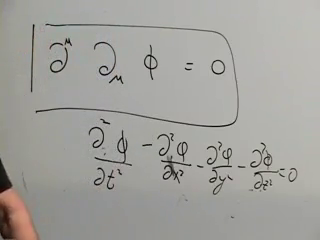
\includegraphics[width=0.75\textwidth]{lecture_07_figure_14.png}
\caption{スカラー波動方程式の縮約された微分形と、その時間マイナス空間の成分展開。}
\lectureframe{01:39:40}
\end{figure}

\begin{classroomqa}
\audiencequestion{波動方程式の右辺はゼロでなければならないのか？}
\lecturerresponse{いいえ。問題と両立する任意のスカラーでよい。\(\phi\) の定数倍や、\(\phi^2\) に比例するような非線形スカラー関数でも、共変性は保たれる。ゼロの場合が最も単純な自由波動方程式を与える。}
\end{classroomqa}

このスカラーの例の要点は準備である。マクスウェル方程式は電場と磁場をより複雑に混ぜ合わせるが、それらもまた、その添字構造からローレンツ不変性が見えるように書くことができる。それが次回に戻る問題である。
